U ovom poglavlju prikazat ćemo analizu kombinatornih igara i matematičku teoriju koja se nalazi u pozadini. 


\section{Analiza igre oduzimanja}

Analizu igre oduzimanja započet ćemo od kraja prema početku. Ako je na hrpi ostao samo jedan, dva ili tri žetona igrač koji je idući na redu pobjeđuje uzimanjem svih preostalih žetona pa su zbog toga te pozicije N-pozicije. 

Sada pretpostavimo da je ostalo četiri žetona. Ako igrač koji miče sljedeći uzme jedan ili dva žetona, protivnik mu može uzvratiti na način da ostavi hrpu sa jednim ili dva žetona, čime on dolazi u poziciju da gubi u igri. Međutim, ako igrač koji miče sljedeći uzme sva tri, ostavlja jedan žeton na hrpi. Tada njegov protivnik mora uzeti preostali žeton, a igrač koji je bio na potezu prije njega pobjeđuje pa je pozicija s 4 žetona P-pozicija.

Ako je na hrpi 5, 6 ili 7 žetona, trenutni igrač može uzeti dovoljno žetona da dovede protivnika u stanje igre u P-poziciju s 4 žetona. To znači da ako igrač uzme x žetona, njegov protivnik će morati uzeti (4 - x) žetona, što će ga dovesti u poziciju s 4 žetona, gdje će izgubiti. Zbog toga su pozicije s 5, 6 ili 7 žetona na hrpi N-pozicije.

Kada se na hrpi nalazi 8 žetona, igrač koji je tada na potezu ne može ostaviti protivnika u P-poziciji s 4 žetona, što znači da je stanje igre s 8 žetona na hrpi klasificirano kao P-pozicija.

Slično kao u navedenim primjerima, možemo izvesti prikaz P i N pozicija za svako stanje igre pa tako dolazimo do prikaza svih P i N pozicija u igri oduzimanja.

\begin{comment}

\begin{table}[H]
\caption{Prikaz P-pozicija i N-pozicija u igri oduzimanja}
\label{tbl:igra21}
\centering
\begin{tabular}{|c|c|c|c|c|c|c|c|c|c|c|c|c|c|c|c|c|c|c|c|c|c|}
\hline
0 & 1 & 2 & 3 & 4 & 5 & 6 & 7 & 8 & 9 & 10 & 11 & 12 & 13 & 14 & 15 & 16 & 17 & 18 & 19 & 20 & 21 \\
\hline
P & N & N & N & P & N & N & N & P & N & N & N & P & N & N & N & P & N & N & N & P & N \\
\hline
\end{tabular}
\end{table}

\end{comment}

\begin{table}[H]
\caption{Prikaz P-pozicija i N-pozicija u igri oduzimanja (1-11)}
\label{tbl:igra21_1-11}
\centering
\begin{tabular}{|c|c|c|c|c|c|c|c|c|c|c|c|}
\hline
0 & 1 & 2 & 3 & 4 & 5 & 6 & 7 & 8 & 9 & 10 & 11 \\
\hline
P & N & N & N & P & N & N & N & P & N & N & N \\
\hline
\end{tabular}
\end{table}


\begin{table}[H]
\caption{Prikaz P-pozicija i N-pozicija u igri oduzimanja(12-21)}
\label{tbl:igra21_12-21}
\centering
\begin{tabular}{|c|c|c|c|c|c|c|c|c|c|c|c|c|c|c|c|c|c|c|c|c|c|}
\hline
12 & 13 & 14 & 15 & 16 & 17 & 18 & 19 & 20 & 21 \\
\hline
P & N & N & N & P & N & N & N & P & N \\
\hline
\end{tabular}
\end{table}

Kao zaključak ove analize, možemo vrlo jednostavno definirati ova dva pravila:

\begin{enumerate}
\item Pozicija s koje je moguće pomaknuti se na P-poziciju je N-pozicija.
\item Ako je trenutna pozicija ona s koje se ne može doći do P-pozicije (to jest, svi su mogući potezi na N-pozicijama) ili ako nema više mogućih poteza, onda je to P-pozicija. 
\end{enumerate}

Lako je zaključiti da je svaka pozicija s n žetona, gdje je n = 4k, P-pozicija, a sve ostale pozicije (n = 4k + 1, n = 4k + 2, n = 4k + 3) su N-pozicije. Logičan dokaz toga jest činjenica da postoji potez od svakog broja koji nije djeljiv s 4 do onog koji je djeljiv s 4 (uzimajući jedan žeton u poziciji 4k + 1, dva žetona u poziciji 4k + 2 ili tri žetona u poziciji 4k + 3). 

Kada oba igrača primjete da je jasno od početka tko će biti pobjednik i da nakon prvog poteza samo izmjenjuju poteze, gdje jedan od njih uzima bilo koji broj žetona, a drugi odgovara tako da uzme ostatak od 4 igra postaje nezanimljiva, zbog čega ćemo u daljnjoj analizi nadograditi ovu igru tako što ćemo odvojiti žetone na više hrpa u igri Nim.

Analiza obrnutog oblika ove igre (misère) nije nimalo zahtjevnija od klasičnog oblika. U misère formi prisiljava se protivnika da mu na kraju ostane jedan žeton u posljednjem potezu, umjesto nijednog. Stoga su P-pozicije n = 4k + 1, a N-pozicije n = 4k, n = 4k + 2 i n = 4k + 3, a igrač koji započinje prvi je gubitnik.



\section{Analiza igre Nim}

\subsection*{N, P pozicije u igri Nim}

Slično kao i u igri oduzimanja, pronalaženje najbolje strategije za pobjedu započinje od završne, terminalne pozicije. To je pozicija u kojoj nema više žetona na ploči za igru. Ova pozicija može se ostvariti samo iz pozicije s jednom hrpom na kojoj se nalazi bilo koji broj žetona pa je pozicija s jednom hrpom N-pozicija. 

Igra s dvije hrpe nije nimalo kompliciranija. Prvi igrač bira hoće li ukloniti jedan žeton sa lijeve hrpe, jedan žeton sa desne hrpe ili oba žetona s desne hrpe. Ako ukloni samo jedan žeton s desne hrpe na kojoj se nalaze dva žetona protivnik će morati ukloniti jedan od preostalih žetona pa će prvi igrač pobijediti. U suprotnom, ukloni li prvi igrač oba žetona ili žeton s lijeve hrpe omogućit će protivniku pobjedu.

\begin{figure}[H]
\centering
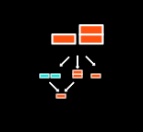
\includegraphics[]{slike-analiza/slika1.png}
\caption{Prikaz igre sa dvije hrpe.}
\label{}
\end{figure}


Sada razmotrimo malo zahtjevniji primjer, kada se u igri nalaze tri hrpe sa po jednim, dva i tri žetona. Pristup pronalaženju najboljih poteza ostaje isti. Uzmimo primjer najjednostavnije pozicije s tri hrpe, (1,1,1), kada se na svakoj od tri hrpe nalazi po jedan žeton. Vrlo je jednostavno zaključiti da u toj poziciji pobjeđuje prvi igrač jer ne postoji niti jedan potez koji bi omogućio drugom igraču da ostvari pobjedu. Zbog toga je pozicija (1,1,1) N-pozicija.

\begin{figure}[H]
\centering
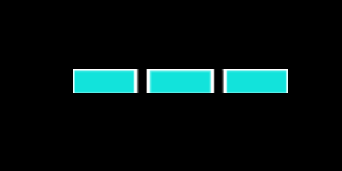
\includegraphics[]{slike-analiza/slika2.png}
\caption{Prikaz pozicije s jednim žetonom na svakoj hrpi.}
\label{}
\end{figure}

Sljedeća pozicija koju bismo analizirali je pozicija (1,1,2). Postoje tri moguća poteza koje igrač može odigrati iz ove pozicije: (1,1), (1,2) ili (1,1,1). Pozicija (1,2) je također N-pozicija jer igrač koji je tada na potezu može odigrati potez koji će poziciju pretvoriti u (1,1), što je N-pozicija. Pozicija (1,1,1) je također N-pozicija, kao što smo već vidjeli. Ostaje nam razmotriti poziciju (1,1), koja predstavlja P-poziciju jer se radi o igri s dvije hrpe jednake veličine. S obzirom da postoji potez koji vodi iz pozicije (1,1,2) u P-poziciju (1,1), poziciju (1,1,2) također možemo proglasiti N-pozicijom.


\begin{figure}[H]
\centering
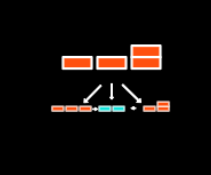
\includegraphics[]{slike-analiza/slika3.png}
\caption{Prikaz mogućih poteza iz pozicije (1,1,2).}
\label{}
\end{figure}

Sada ćemo analizirati poziciju (1,2,2). Svi mogući potezi iz ove pozicije su (1,1,2), (1,2) i (2,2). Pozicija (1,1,2) i pozicija (1,2) su N-pozicije, dok je pozicija (2,2) P-pozicija jer se radi o igri s dvije hrpe iste veličine. S obzirom da su svi mogući potezi iz pozicije (1,2,2) N-potezi, poziciju (1,2,2) također možemo proglasiti N-pozicijom.

Za analizu pozicije (1,2,3), postoji šest mogućih poteza. Pozicija (1,2) se identificira kao N-pozicija jer se može reducirati na (1,1) i (1,2) koje su obje N-pozicije. Pozicija (1,1,2) također je N-pozicija jer se može reducirati na (1,1) i (2), obje N-pozicije. 
Pozicija (1,2,2) je N-pozicija jer se može reducirati na (1,2) i (2), obje N-pozicije. Na isti način reduciramo pozicije (1,1,3) na (1,3) i (1,1,1), (1,3) na (1,2) i (1), (2,3) na (1,2) i (1,1).
 
Kada se sve pozicije analiziraju, može se napraviti stablo svih mogućih pozicija, koje pokazuje da se oba gore navedena pravila mogu primjeniti na igru Nim s tri hrpe: svaka P-pozicija ima samo djecu pozicije koje su N-pozicije, a svaka N-pozicija ima barem jedno dijete koje je P-pozicija. Na slici je svaka P-pozicija prikazana plavom bojom, a N-pozicija crvenom bojom.

\begin{figure}[H]
\centering
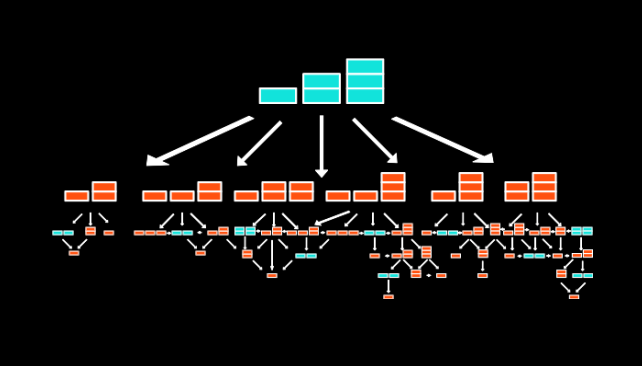
\includegraphics[]{slike-analiza/slika4.png}
\caption{Stablo svih mogućih pozicija u igri Nim s tri hrpe.}
\label{}
\end{figure}

Ako se ova analiza proširi na igru s više hrpa, proces pronalaženja P i N-pozicija postaje složeniji, ali osnovni principi ostaju nepromjenjeni. 



\subsection*{Nim vrijednost}

Svaku P i N-poziciju u igri Nim moguće je dobiti analizom u prethodnom poglavlju, no postavlja se pitanje praktičnosti analize igara s više hrpa, a samim time i većim veličinama hrpa. Zbog toga moramo uvesti bolje načine analize pozicija u igri Nim.

Jedan od novih i boljih načina analiza pozicija u igri Nim predstavili su matematičari Roland P. Sprague i Patrick M. Grundy.\cite{2008gametheoryferguson} Oni koriste binarne brojeve za opisivanje svakog stanja igre Nim, pri čemu se dekadski broj žetona na svakoj hrpi prebacuje u binarni oblik. Ukupna vrijednost pozicije nije samo vrijednost jedne hrpe, nego zbroj svih binarnih vrijednosti.

Definicija Nim zbrajanja glasi:
\begin{definition}
(x\textsubscript{n} x\textsubscript{n-1} $\dots$ x\textsubscript{1} x\textsubscript{0}) $\oplus$ (y\textsubscript{n} y\textsubscript{n-1} $\dots$ y\textsubscript{1} y\textsubscript{0}) = (z\textsubscript{n} z\textsubscript{n-1} $\dots$ z\textsubscript{1} z\textsubscript{0}), gdje je svaki z = (x + y) mod 2.
\end{definition}

Pomoću ove definicije možemo za svaku poziciju odrediti njezin Nim zbroj. No kako odrediti je li ta pozicija P-pozicija ili N-pozicija? Uzmimo ponovno za primjer igru Nim sa tri hrpe iz gornjeg primjera. Pretvorbom dekadske vrijednosti broja žetona na svakoj hrpi u binarni oblik dobivamo vrijednosti 1, 10 i 11.
Nim zbroj tih binarnih vrijednosti daje rezultat 0.

\begin{center}
1 = (\texttt{1})\textsubscript{2}\newline
2 = (\texttt{10})\textsubscript{2}\newline
3 = (\texttt{11})\textsubscript{2}\newline
\rule{2cm}{0.1pt}\newline
$\oplus$ = (\texttt{00})\textsubscript{2}\newline
\end{center}

Iz gornjeg primjera već znamo da je ta pozicija P-pozicija. Uzmimo sada kao primjer poziciju (1,2,2), za koju već znamo da je N-pozicija. Pretvorbom dekadskih vrijednosti u binarni oblik i Nim zbrajanjem dobivamo vrijednost 100.

\begin{center}
1 = (\texttt{1})\textsubscript{2}\newline
2 = (\texttt{10})\textsubscript{2}\newline
2 = (\texttt{10})\textsubscript{2}\newline
\rule{2cm}{0.1pt}\newline
$\oplus$ = (\texttt{01})\textsubscript{2}\newline
\end{center}

Na temelju navedenih primjera možemo zaključiti da su sve P-pozicije u igri Nim vrijednosti jednake 0, dok su sve N-pozicije u igri Nim vrijednosti različite od 0. To se može izraziti kroz sljedeći korolar.

\begin{korolar}\cite{tucker2002appliedcombinatorics}
Pozicija (x\textsubscript{1}, $\dots$, x\textsubscript{n}), n $\in$ N  je P-pozicija ako i samo ako
x\textsubscript{1} $\oplus$ $\dots$ $\oplus$ x\textsubscript{n} = 0
\end{korolar}

Funkcionalnosti ove dvije obrađene metode mogu se činiti sličnima, no analiza Nim vrijednosti ima veliki utjecaj tijekom igranja igre jer pruža brzu i jednostavnu metodu pronalaženja najboljeg poteza iz bilo koje pozicije u igri. Dok N-pozicije i P-pozicije pokazuju samo karakter trenutne pozicije bez metode određivanja kako odabrati najbolji mogući potez, pomoću Nim vrijednosti lako se može odrediti najbolja opcija za kretanje kroz igru.

Na primjer, zamislimo igru Nim sa tri hrpe koja ima više od tri žetona na svakoj hrpi. Uzmimo za primjer da su količine žetona na svakoj hrpi 25, 21 i 10. Pomoću N-pozicija i P-pozicija teško ćemo odrediti koji potez odigrati, no pomoću Nim vrijednosti to možemo vrlo lako učiniti. Pretvorbom u binarni oblik dobivamo vrijednosti 11001, 10101 i 1010, a Nim zbrajanjem dobivamo vrijednost 6, što je N-pozicija.

\begin{center}
25 = (\texttt{11001})\textsubscript{2}\newline
21 = (\texttt{10101})\textsubscript{2}\newline
10 = (\texttt{1010})\textsubscript{2}\newline
\rule{2cm}{0.1pt}\newline
$\oplus$ = (\texttt{100})\textsubscript{2}\newline
\end{center}

Najbolji izbor za igrača na potezu bi trebao biti svaki potez koji ima vrijednost Nim zbroja 0, što može lako napraviti ako pogleda zapis zbroja. Na primjer može uzeti dva žetona sa hrpe koja ima 21 žeton, što odmah mijenja Nim vrijednost u 0. Taj potez ostavlja protivnika u gubitničkoj poziciji i omogućava prvom igraču da dođe do pobjedničke pozicije.

\begin{center}
25 = (\texttt{11001})\textsubscript{2}\newline
19 = (\texttt{10011})\textsubscript{2}\newline
10 = (\texttt{1010})\textsubscript{2}\newline
\rule{2cm}{0.1pt}\newline
$\oplus$ = (\texttt{000})\textsubscript{2}\newline
\end{center}


\subsection*{Sprague-Grundyjeva funkcija}

Općenitiji način za analizu nepristrane igre je korištenje Sprague-Grundyjeve funkcije (S-G funkcija)\cite{1939mathematicsandgames} \cite{1973ubermathematischekampfspiele}. Prvo moramo upotrijebiti neke nove zapise koji općenito opisuju nepristrane igre kako bi se kasnije mogla definirati sama S-G funkcija. Ovaj novi zapis bit će predstavljen parom (X, F), gdje X označava sve pozicije u igri, a F je funkcija koja definira sve moguće pozicije x $\in$ X. Zbog činjenice da se svi potezi uvijek izvode iz jedne pozicije igre na skup pozicija, funkcija F nam daje podskup F(x) od X na svaku poziciju x $\in$ X. Drugim riječima, ova funkcija dodjeljuje sve dostupne pozicije za bilo koju odabranu poziciju u igri.

Formalna definicija Sprague-Grundyjeve funkcije slijedi u nastavku:

\begin{definition}\cite{2008gametheoryferguson}
    Sprague-Grundyjeva funkcija grafa (X, F) je funkcija g, definirana na skupu X, koja uzima nenegativne cjelobrojne vrijednosti, pri čemu vrijedi:

\begin{center}
    g(x) = min (n $\geq$ 0 : n $\neq$ g(y), y $in$ F(x))
\end{center}

\end{definition}

Sama definicija na prvi pogled izgleda poprilično zbunjujuća zbog korištenja rekurzije u definiciji. Međutim, algoritam postaje vrlo jednostavan za razumijevanje i primjenu kada se počne graditi od završne, terminalne pozicije. Sve terminalne pozicije imaju vrijednost 0, a skup F(x) je prazan. Vrijednost g od terminalnog položaja tada se dodjeljuje kao broj jednak minimalnoj vrijednosti skupa n $\in$ \{0, 1, 2...\}, što je 0. Uzimajući u obzir poziciju čiji je jedini sljedbenik terminalna pozicija, vrijednost funkcije postaje g(x) = 1.

Iz ovih uvjeta slijedi da je pozicija x P-pozicija ako je vrijednost Sprague-Grundyjeve funkcije 0, inače su sve ostale pozicije N-pozicije:

\begin{itemize}
    \item Ako je x terminalna pozicija, tada je g(x) = 0.
    \item Za poziciju x za koju je g(x) = 0, svi su sljedbenici y od x takvi da je g(y) $\neq$ 0.
    \item Za poziciju x za koju je g(x) $\neq$ 0, postoji barem jedan sljedbenik y za koji je g(y) = 0.
\end{itemize}

Iz tih uvjeta možemo izvesti iduću propoziciju:

\begin{proposition}
Ako je vrijednost funkcije g(x) jednaka 0 za određeni vrh x $\in$ X, tada se vrh x označava kao P-vrh na grafu.
\end{proposition}

Iz tih uvjeta lako možemo vidjeti da postoji sličnost u funkcionalnosti između analize pomoću S-G funkcije i analize P-pozicija i N-pozicija. Procjena prema N-pozicijama i P-pozicijama označava sva stanja koja mogu dosegnuti P-poziciju iz N-pozicije, dok S-G funkcija svemu tome dodjeljuje broj različit od 0. S druge strane, P-pozicija je definirana kao ona čiji su jedini sljedbenici N-pozicije, što se izražava S-G vrijednošću 0 i kao ona pozicija sa sljedbenicima S-G vrijednosti različitih od 0.




Kako bismo analizu kombinatornih igara učinili što pristupačnijom i kao rezultat cjelokupne teorijske analize, u idućim poglavljima analizirat ćemo izrađenu interaktivnu web aplikaciju koja implementira jednu verziju igre Nim. To će omogućiti korisnicima da eksperimentiraju s igrom i bolje usavrše razumijevanje koncepata igre o kojima se govori u ovom radu.